\chapter{THỰC THI VÀ ĐÁNH GIÁ THỰC NGHIỆM}

\section{Xây dựng môi trường và triển khai}

\quad TourXport được đóng gói trong các container thông qua công nghệ Docker Compose \cite{docker_compose}, đảm bảo tính nhất quán tuyệt đối về cấu hình môi trường từ máy phát triển cục bộ đến máy chủ thực tế. Tập lệnh docker-compose.yml định nghĩa hạ tầng triển khai song song ba dịch vụ độc lập:

\begin{itemize}
    \item \textbf{Dịch vụ backend}: Triển khai trên môi trường Node.js (Express.js) \cite{nodejs,expressjs} (cổng 3000), thực hiện volume mapping với mã nguồn tại thư mục ./backend và sử dụng công cụ nodemon để tự động nạp lại khi có sự thay đổi mã nguồn.
    
    \item \textbf{Dịch vụ ai\_backend (AI Worker)}: Triển khai môi trường Python 3.10-slim (cổng 8000). Tập lệnh Dockerfile tự động hóa quá trình cài đặt phụ thuộc từ requirements.txt và khởi chạy máy chủ Uvicorn. Dịch vụ này cũng áp dụng cơ chế watch mode để đồng bộ tự động mã nguồn từ thư mục src/ vào bộ chứa. ai\_backend chỉ được expose qua port 8000 nội bộ của Docker, nên chỉ mỗi backend Node.js mới giao tiếp được với ai\_backend.
    
    \item \textbf{Frontend (Flutter)}: Được biên dịch và khởi chạy trực tiếp trên thiết bị thực tế hoặc máy ảo thông qua công cụ dòng lệnh flutter run. Ứng dụng client sẽ giao tiếp với cụm máy chủ thông qua các kiến trúc RESTful API.
\end{itemize}

\section{Kết quả thực thi các Use Case}

\subsection{Use Case Đăng nhập và Xác thực}

\begin{figure}[H]
    \centering
    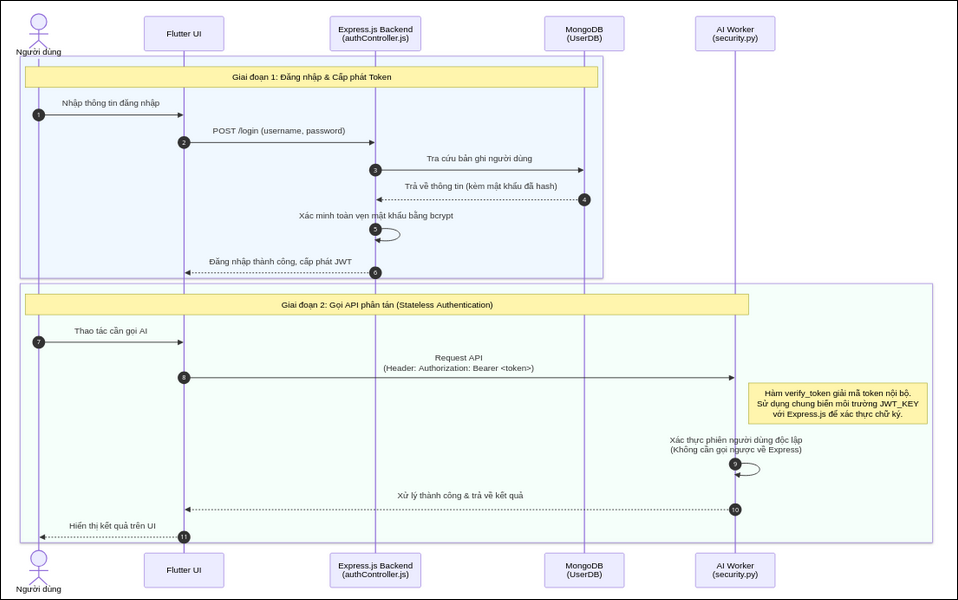
\includegraphics[width=1\textwidth]{img/C4-1.png}
    \caption{Sequence Diagram mô tả use case Đăng nhập và xác thực}
\end{figure}

\quad Khi người dùng gửi thông tin đăng nhập qua giao diện Flutter, Backend Express.js (tại authController.js, hàm login) sẽ tiến hành tra cứu bản ghi trong tập hợp UserDB và xác minh tính toàn vẹn của mật khẩu bằng thuật toán mã hóa bcrypt. Khi đăng nhập thành công, hệ thống cấp phát một JSON Web Token (JWT).

\quad Token này sau đó được gắn vào header của giao thức HTTP (Authorization: Bearer <token>) cho mọi yêu cầu (request) về sau. Điểm đáng chú ý trong kiến trúc phân tán là khi người dùng gọi API của AI Worker, hệ thống AI tự động áp dụng hàm verify\_token (ai\_backend/src/core/security.py) để giải mã token nội bộ. Do AI Worker sử dụng chung một khóa bí mật (biến môi trường JWT\_KEY) với Backend Express.js, nó có thể xác thực được phiên người dùng mà không cần phải gọi API ngược về Backend Express.js, giúp giảm chi phí độ trễ (latency).

\subsection{Use Case Khảo sát nhu cầu người dùng (Survey)}

\quad Trong giai đoạn POC hiện tại, quy trình của Use Case này đang tập trung vào việc xây dựng trải nghiệm thu thập thông tin người dùng ở phía Frontend. Cụ thể, ứng dụng Flutter đã hoàn thiện thiết kế giao diện khảo sát (Survey Screen), cho phép du khách nhập các thông số đầu vào cần thiết cho chuyến đi, bao gồm:

\begin{itemize}
    \item Ngân sách tối đa.
    \item Số ngày dự kiến.
    \item Các sở thích cá nhân cụ thể.
\end{itemize}

\quad Hiện tại, hệ thống đã hoàn tất phần thiết kế UI/UX và các logic quản lý trạng thái biểu mẫu (form state management) trên thiết bị người dùng. Bước tích hợp (Integration) để đóng gói dữ liệu này dưới định dạng JSON và thực hiện lời gọi API thực tế tới endpoint POST /api/trip/generate của AI Worker đang trong lộ trình phát triển và sẽ được hoàn thiện ở các bản cập nhật tiếp theo.

\begin{figure}[H]
    \centering
    \begin{minipage}[t]{0.3\textwidth}
        \centering
        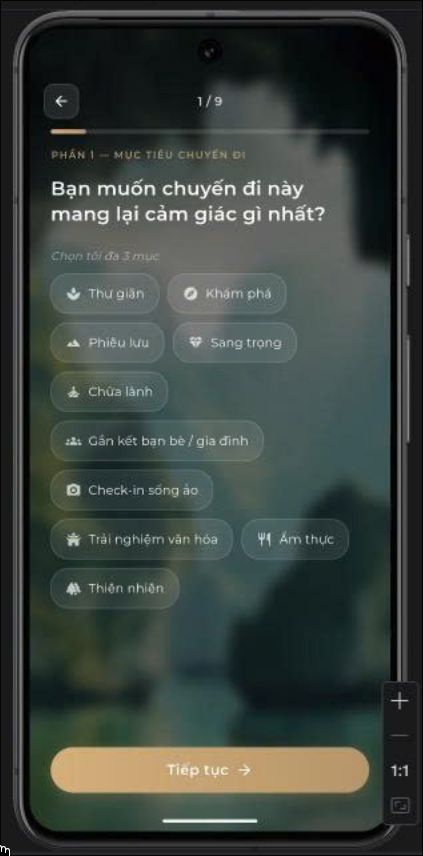
\includegraphics[width=\textwidth]{img/C4-2.png}
    \end{minipage}
    \hfill
    \begin{minipage}[t]{0.294\textwidth}
        \centering
        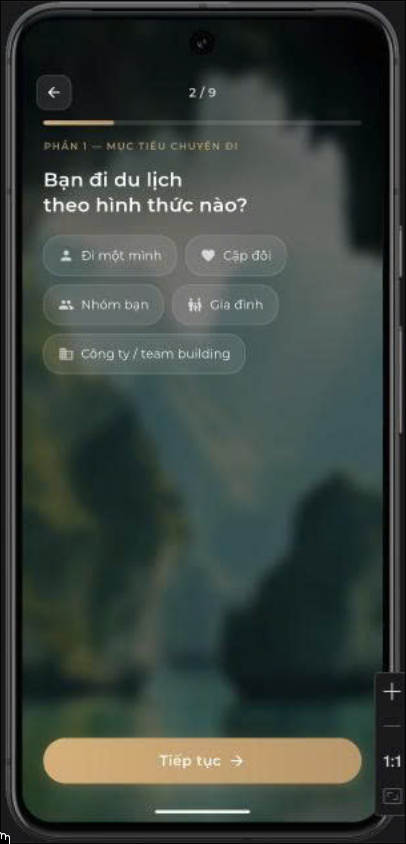
\includegraphics[width=\textwidth]{img/C4-3.png}
    \end{minipage}
    \hfill
    \begin{minipage}[t]{0.29\textwidth}
        \centering
        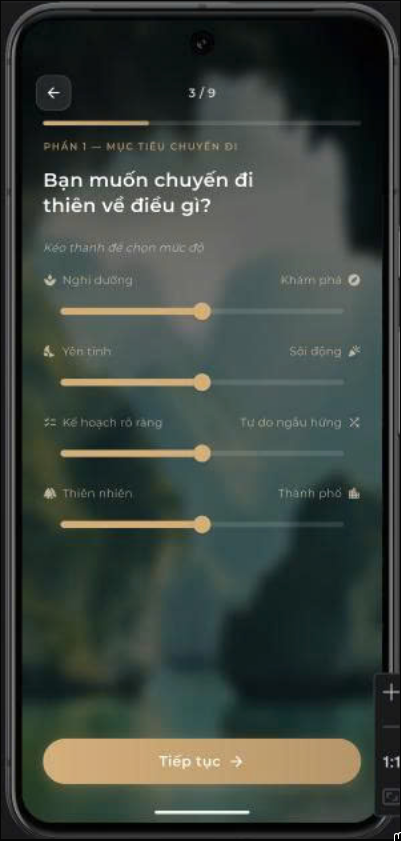
\includegraphics[width=\textwidth]{img/C4-4.png}
    \end{minipage}
    \caption{Màn hình câu hỏi Survey - Mô phỏng trên máy ảo Android}
\end{figure}

\quad Tuy quy trình end-to-end từ Frontend đến Backend chưa được liên kết, toàn bộ luồng xử lý lõi ở phía máy chủ (server-side) đã được xây dựng và kiểm thử độc lập thành công. Khi Frontend sẵn sàng gửi dữ liệu, AI Worker đã có sẵn cơ chế kiểm duyệt dữ liệu tự động thông qua mô hình Pydantic (TripGenerateRequest tại ai\_backend/src/schemas/request/trip\_generator.py). Các request vi phạm điều kiện logic, như ngân sách âm hoặc số ngày vượt quá ngưỡng 30, sẽ bị từ chối ngay lập tức tại cổng API kèm mã lỗi 422 Unprocessable Entity. Khi nhận dữ liệu hợp lệ, luồng Orchestrator sẽ kết nối với OpenAI để sinh ra danh sách các hoạt động du lịch (Location) được phân bổ theo ngày và buổi, tạo tiền đề để Frontend render giao diện timeline sau này.

\begin{figure}[H]
    \centering
    
\includegraphics[width=0.3\textwidth]{img/C4-5.png}
    \caption{Kết quả từ Survey - Mô phỏng trên máy ảo Android}
\end{figure}

\subsection{Đánh giá độ chính xác và hiệu năng hệ thống}

\subsubsection{Hiệu năng hệ thống và độ trễ}

\quad Hệ thống thể hiện hiệu năng tổng thể ổn định và tối ưu xuyên suốt các tầng kiến trúc. Ở phía Client, Frontend Flutter vận hành mượt mà trên đa nền tảng nhờ engine kết xuất đồ họa hiệu năng cao, quản lý trạng thái hiệu quả giúp UI không bị gián đoạn ngay cả khi hiển thị các dữ liệu phức tạp. Tại Server-side, Backend Node.js (Express) xử lý các tác vụ IO chuyên sâu, như truy vấn dữ liệu địa điểm và xác thực người dùng, với độ trễ cực thấp nhờ cơ chế non-blocking I/O.

\quad Đối với hệ thống AI Worker (FastAPI), việc sử dụng hoàn toàn luồng xử lý bất đồng bộ (Asyncio kết hợp thư viện AsyncOpenAI và Motor) giúp giải quyết triệt để nút thắt cổ chai hệ thống. Hiện tại, độ trễ lớn nhất của hệ thống chủ yếu phụ thuộc vào thời gian xử lý tự nhiên của OpenAI API, dao động từ 2 đến 5 giây tùy vào độ dài prompt, trong khi các thành phần nội bộ đều phản hồi gần như tức thời.

\subsubsection{Độ chính xác và tính toàn vẹn dữ liệu}

\quad Dữ liệu của dự án được bảo vệ và kiểm duyệt qua nhiều lớp. Trên Frontend, người dùng bị ràng buộc bởi các form validation, như nhập đúng định dạng email và ngân sách. Khi dữ liệu đến Backend Express, tính toàn vẹn tiếp tục được đảm bảo thông qua hệ thống Mongoose Schema, ví dụ UserDB ép buộc tính duy nhất của email và số điện thoại, bcrypt băm mật khẩu an toàn.

\quad Đối với luồng sinh dữ liệu bằng trí tuệ nhân tạo, hệ thống khắc phục hoàn toàn điểm yếu phổ biến của LLM là trả về JSON bị hỏng (malformed data). Nhờ áp dụng tính năng Structured Outputs của OpenAI kết hợp với cơ chế validate và parse chặt chẽ của Pydantic, tỷ lệ lỗi format kết quả giảm xuống ngưỡng tiệm cận 0%. Các kiểu dữ liệu khó kiểm soát, như số thực float cho chi phí và UUID của địa điểm, luôn được định dạng chính xác tuyệt đối theo API Contract.

\subsubsection{Tính mô-đun và khả năng mở rộng}

\quad Việc thiết kế kiến trúc phân tán (Microservices-oriented) phân tách rạch ròi giữa UI (Flutter), Logic quản trị lõi (Express.js), AI Engine (FastAPI) và Cơ sở dữ liệu tập trung (MongoDB Atlas) mang lại khả năng mở rộng độc lập tuyệt vời. Khi phát sinh trường hợp lưu lượng người dùng yêu cầu sinh lịch trình tăng đột biến, quản trị viên chỉ cần cấp phát thêm tài nguyên riêng cho các container của dịch vụ AI Worker.

\quad Quá trình này diễn ra hoàn toàn biệt lập, không gây ảnh hưởng đến phần lõi quản lý thông tin người dùng hay truy xuất dữ liệu đang vận hành trên cụm Node.js. Song song đó, việc chọn MongoDB làm kho lưu trữ tập trung giúp cả hai backend, Node.js và Python, có thể giao tiếp và truy xuất khối lượng lớn dữ liệu phi cấu trúc một cách linh hoạt, tạo bản lề vững chắc cho việc triển khai các hệ thống phức tạp hơn như RAG (Retrieval-Augmented Generation) trong tương lai.
